
\begin{frame}{What is the power of HML}
 \Margines{
 \vspace{-0.5cm}
 {\bf Question:}\  What are the trees that can be distinguished using HML? 
 %And what is the power of $HML+ predicates\ p_1\ldots$?
 
 \begin{itemize}
 \item<2-> What can we distinguish by formulas with modal depth 1.
 \item<3-> What can we distinguish by formulas with modal depth 2.
 \item<4-> What can we distinguish by formulas with modal depth 3.
 \item<5-> What can we distinguish by formulas with modal depth 4.
 \end{itemize}


 \visible<6->{
 \alt<7>
 {
 {\bf Labelled case:}
  \begin{definition}
  Bisimulation $B$ is any relation on a set of configurations (nodes) that satisfies following conditions 
  \begin{enumerate}
   \item \red{if $(s,s')\in B$ then $L(s)=L(s'),$}
   \item if $(s,s')\in B$ then for every $t$ such that $s\to t$ there is $t'$ such that $s'\to t'$ and $(t,t')\in B$, 
   \item if $(s,s')\in B$ then for every $t'$ such that $s'\to t'$ there is $t$ such that $s\to t$ and $(t,t')\in B$.
  \end{enumerate}
 We denote it by $s \sim_B s'$.
 \end{definition}
 }
 {{\bf Unlabelled case:}
 \begin{definition}{}
  Bisimulation $B$ is any relation on a set of configurations (nodes) that satisfies following conditions
  \begin{enumerate}
   \item if $(s,s')\in B$ then for every $t$ such that $s\to t$ there is $t'$ such that $s'\to t'$ and $(t,t')\in B$, 
   \item if $(s,s')\in B$ then for every $t'$ such that $s'\to t'$ there is $t$ such that $s\to t$ and $(t,t')\in B$.
  \end{enumerate}
  We denote it by $s \sim_B s'$.
 \end{definition}
}
}
 }
\end{frame}

\begin{frame}{Bisimulation relation}
 \Margines{

 \begin{theorem}
  A pair of configurations $(s,s')$ can not be distinguished by HML formula if and only if there is a bisimulation relation $B$ such that $s\sim_B s'$. 
 \end{theorem}
 
 We need a few lemmas.

 \visible<2->{\begin{lemma}
  Union of bisimulations is a bisimulation.
 \end{lemma}
 }
 \visible<3-5>{\alt<3>{\begin{block}{Corollary}
  There is a biggest bisimulation.
 \end{block} }{
  \begin{definition}
   \begin{itemize}
    \item The biggest bisimulation is called the bisimilarity relation and denoted by $\sim$.
    \item  We say that two configurations $(s,s')$ are bisimilar if $s\sim s'$.
   \end{itemize}
  \end{definition}
  \begin{itemize}
   \item<5>   Bisimilarity is an equivalence relation.
  \end{itemize}


}
}
}
\end{frame}

\begin{frame}{The proof of the theorem (idea).}
\Margines{
    \begin{block}{$\xrightarrow{}$}
        \begin{enumerate}
            \item  By negation, suppose there is a formula $\phi$ that distinguish $(s,s')$, we prove that $(s,s')$ is not en element of any bisimulation relation.
            \item By induction on the modal depth of the formula.
        \end{enumerate}
    \end{block}
    
    \begin{block}{$\xleftarrow{}$}
    \begin{enumerate}
        \item By induction on the modal depth of the formula.    
    \end{enumerate}
       
    \end{block}
}
\end{frame}

\begin{frame}{The proof of the theorem (idea).}
\Margines{
    \begin{block}{$\xrightarrow{}$}
        \begin{enumerate}
            \item  By negation, suppose there is a formula $\phi$ that distinguish $(s,s')$, we prove that $(s,s')$ is not en element of any bisimulation relation.
            \item By induction on the modal depth of the formula.
        \end{enumerate}
    \end{block}
    
    \begin{block}{$\xleftarrow{}$}
    \begin{enumerate}
        \item By induction on the modal depth of the formula.    
    \end{enumerate}
       
    \end{block}
}
\end{frame}

\begin{frame}[fragile]{}
\begin{center}\begin{Large}
		\huge{CTL and CTL*}
              \end{Large}
\end{center}
\end{frame}

\begin{frame}{An extension of HML - CTL}
\Margines{
\begin{Definition}
\begin{enumerate}
    \item A state formula $\phi= tt | \neg \phi_1 | \phi_1\land \phi_2 | p_i| A\alpha | F\alpha$
 
 \item A path formula (restricted LTL) $\alpha = X\phi_1| \phi_1 U \phi_2 | F\phi_1 | G\phi_1$
 
 \item where $\phi$ are state formulas and $\alpha$ are path formulas.
\end{enumerate}
 
\end{Definition}
\begin{block}{Semantics}\
\begin{itemize}
 \item $p_i$ means that the predicate $p_i$ holds in the configuration in which the formula is evaluated (current configuration). 
 \item  $A\alpha$ for every run $r$ starting at the current configuration the formula $\alpha$ holds for $\trace{r}$.
 \item  $F\alpha$ there is a run $r$ starting at the current configuration such that the formula $\alpha$ holds for $\trace{r}$.
\end{itemize}
\end{block}



}
\end{frame}


\begin{frame}{Exercise}
\Margines{
\begin{itemize}
    \item $F \phi = true U \phi$,
    \item $G \phi = \neg (F \neg \phi)$
\end{itemize}

Which of the following pairs of CTL formulas are equivalent?  For those which are not, find a model of one of the pair which is not a model of the other:\footnote{exercise from https://www.win.tue.nl/~andova/education/2IF25/Ex2Solutions.pdf}
\begin{enumerate}
    \item <2-> $EF \phi$ and $EG\phi$,
    \item <3-> $EF\phi \lor EF\tau$ and $EF(\phi \lor \tau$,
    \item <4-> $AF\phi \lor AF\tau$ and $AF(\phi \lor \tau)$,
    \item <5-> $AF\neg \phi$ and $\neg EG \phi$.
\end{enumerate}

\begin{itemize}
    \item<6-> Write a $CTL$ formula which stays that there is always a possibility of braking.
\end{itemize}
 
}
\end{frame}




\begin{frame}{LTL vs. CTL}
\Margines{

\vspace{-0.7cm}

\begin{block}{Evaluation of LTL in a state.}
We consider all traces starting in a given state.
\end{block}

\visible<2->{
\alt<2>{
\begin{block}{ Hypothesis }
LTL and For all fragment of CTL describes the same properties.
\end{block}
}{
\begin{lemma}
There are properties which can be expressed in LTL and can not in CTL and vice versa. 
\end{lemma}
}

\visible<4-10>{
\alt<4-6>{
\DwieKol{0.45}{0.40}
{\visible<6->{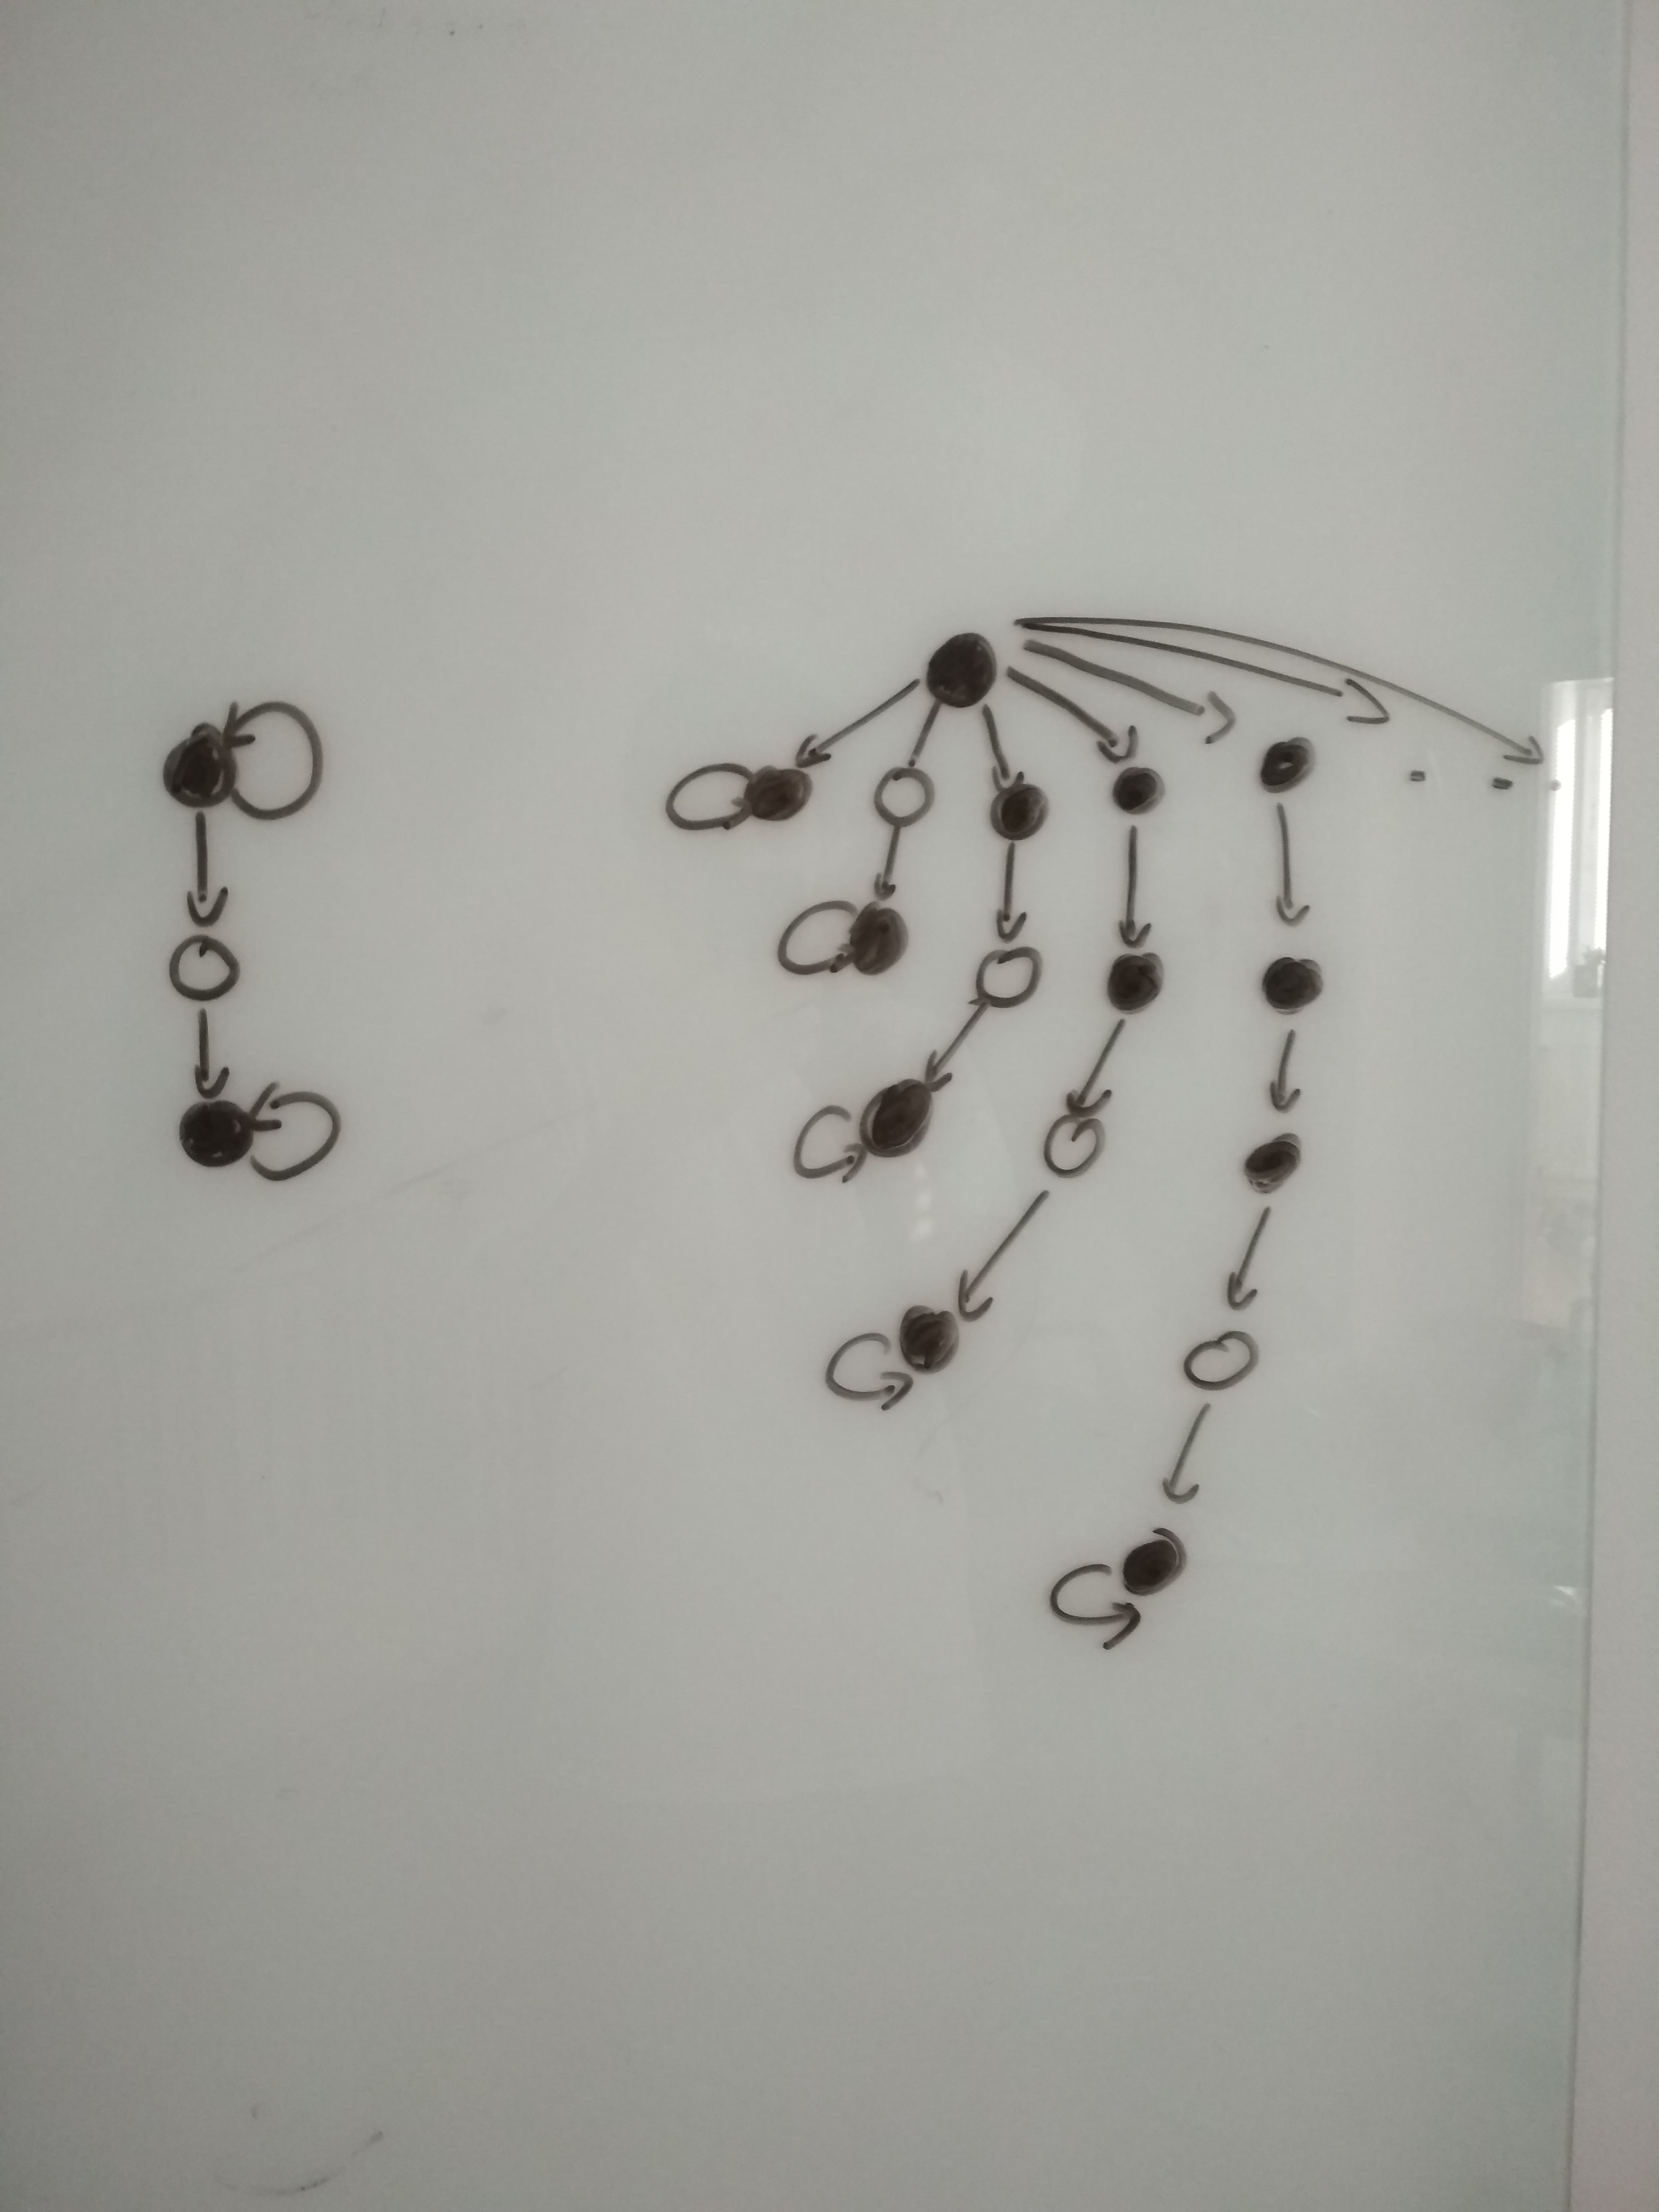
\includegraphics[width=40mm]{CTL not in LTL.jpg}}}
{\vspace{-0cm}
\visible<4->{
\begin{example}[CTL not in LTL]
 A F AG (black == true)
\end{example}}
\visible<5->{
Two systems have the same sets of traces but only one satisfies the formula in CTL.}
}}
{
\begin{example}[LTL not in CTL]
A G F (black = true)\\
For all runs always in the future there will be a moment when lights are on. The idea is to construct two sequences of systems $T_i$ and $T_i'$
such that 

\begin{enumerate}
\item $(T_i,s_0)\models AGF (black = true)$ but
    $(T_i',s_0)\not\models AGF (black = true).$ 
\item $(T_i,s_0)$ and $(T_i',s_0)$ are not distinguished by any CTL formula of the modal depth $i$.
\end{enumerate}
\end{example}

Look: \url{https://www.youtube.com/watch?v=OAf7q3X71-o}
(min 58)

}
}}}
\end{frame}



\begin{frame}{Evaluation of CTL}
 \Margines{
\begin{lemma}
 A CTL formula $\phi$ can be evaluated in time proportional to the length of the formula times size of the Kripke structure.
\end{lemma}

 \begin{proof}
By induction on the derivation tree of the formula. 
 \end{proof}
} 
\end{frame}

\begin{frame}{Bisimulation and CTL}
 \Margines{
 \begin{lemma}
  Two configurations $s$ and $s'$ are bisimilar if and only if $s$ and $s'$ are not distinguished by any $CTL$ formula $\phi$.
 \end{lemma}
 
\visible<2->{
 \begin{block}{Proof $\xleftarrow{}$ }
If they are not distinguishable by CTL, then they are not 
distinguishable by HML, thus they are bisimilar.
 \end{block}
}

\visible<3->{
\begin{block}{Proof $\xrightarrow{}$}
It will be helpful to extend our understanding of bisimulation first. 
\end{block}
}
}
\end{frame}

\begin{frame}{Game characterisation of Bisimilarity}
\Margines{
\vspace{-0.5cm}
\begin{definition}
 A bisimulation game is played in rounds between two players Spoiler and Duplicator. Arena is a set of pairs of configurations of the Kripke structure.
 Suppose that current pair of configurations is $(s,s')$.
 
 Rules of a round are as follows:
 \begin{itemize}
  \item  First Spoiler chooses one of configurations $s$ or $s'$. Without lost of generality we may assume 
that it is $s$.
\item Next he chooses a configuration $t$ such that $s\to t$.
\item Next Duplicator chooses a configuration $t'$ such that $s'\to t'$ where $s'$ is 
a configuration no chosen by Spoiler. 
\item The next round of the game will be plaid from $(t,t').$
 \end{itemize}


Winning conditions:
\begin{itemize}
 \item If $L(s)\neq L(s')$ then Spoiler wins. 
 \item If any player can not make his part of the move then he looses.
 \item Infinite plays are won by Duplicator.
\end{itemize}
\end{definition}
}
\end{frame}

\begin{frame}
\Margines{

\begin{lemma}
 A winning strategy for Spoiler is a tree.
\end{lemma}

\visible<2->{
\begin{lemma}
 Spoiler has a winning strategy in the bisimulation game starting from a pair of configurations $(s,s')$ if and only if $s\not\sim s'$.
\end{lemma}
}



}

 
\end{frame}



\begin{frame}{Bisimulation and CTL}
 \Margines{
 \begin{lemma}
  Two configurations $s$ and $s'$ are bisimilar if and only if $s$ and $s'$ are not distinguished by any $CTL$ formula $\phi$.
 \end{lemma}
 
\visible<2->{
\begin{block}{Proof $\xrightarrow{}$}
If they are distinguishable by CTL, then they are distinguishable by some formula.
We prove via induction on the modal depth of the formula.
\end{block}
}
}
\end{frame}



\begin{frame}{Extend even more - $CTL^*$}
\Margines{
\begin{Definition}
 A state formula $\phi= tt | \neg \phi_1 | \phi_1\land \phi_2 | p_i| A\alpha | F\alpha$
 
 A path formula (restricted LTL) $\alpha = \phi| \neg \alpha_1| \alpha_1\land \alpha_2| X\alpha_1| \alpha_1 U \alpha_2 $
\end{Definition}
\begin{block}{Semantics}\
\begin{itemize}
 \item  $A\alpha$ for every run $r$ starting at the current configuration the formula $\alpha$ holds for $\trace{r}$.
 \item  $F\alpha$ there is a run $r$ starting at the current configuration such that the formula $\alpha$ holds for $\trace{r}$.
\end{itemize}
\end{block}

\begin{block}{Fact}
$CTL^*$ subsumes CTL and LTL.
\end{block}}
\end{frame}


\begin{frame}{Bibliography}
\Margines{
 CTL, CTL* 
 
 \url{https://www.youtube.com/channel/UCUXDMaaobCO1He1HBiFZnPQ}\\
 
 
 Unites: 9, 10, 11.
 
 
 Bisimulation + CTL and more:\\
 \url{https://pdfs.semanticscholar.org/cb9f/325389bd6ee5894dcf435159d34f9e20da2d.pdf}
 }
\end{frame}










